\section{Sensibility Testbed Design}\label{sec-design}

This section describes the design of Sensibility Testbed. On one
hand, Sensibility Testbed manages how device owners make their
devices accessible to the research community. On the other hand,
it offers technical resources to researchers that allow them to
securely collect data from remote mobile devices.

\subsection{Overview}

\begin{figure}
\center{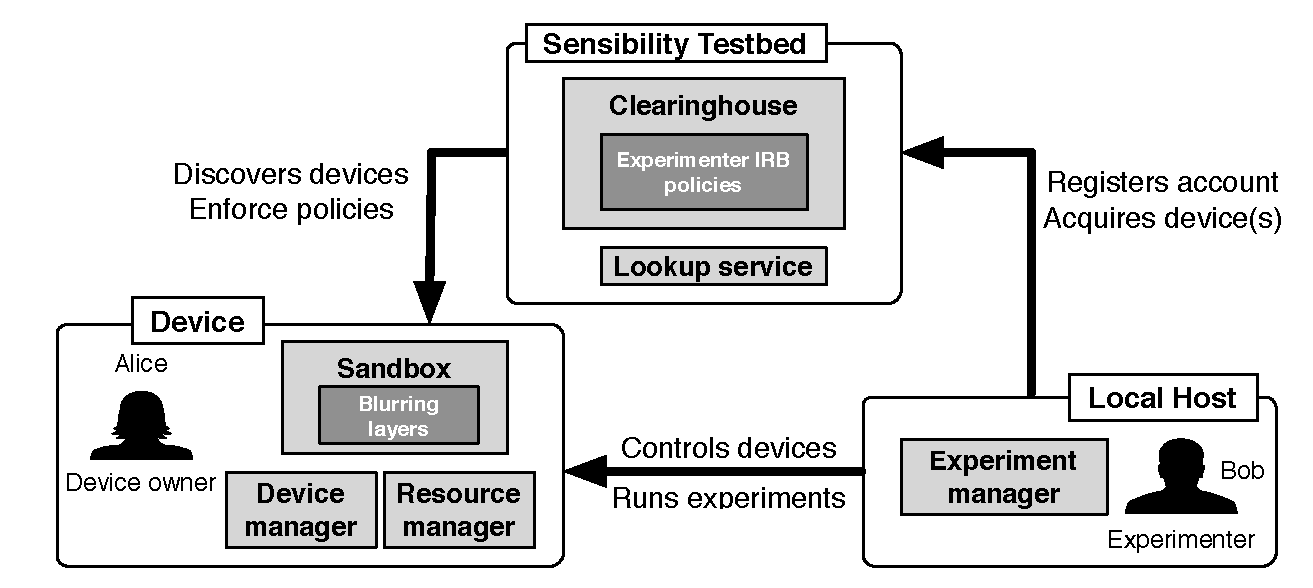
\includegraphics[width=\columnwidth]{figs/arch.pdf}}
%\vspace*{-20pt}
\caption{\small Sensibility Testbed architecture. \yanyan{need 
to replot this diagram.}
\label{fig-arch}}
\end{figure}

\textbf{Interacting parties.}
In Sensibility Testbed, there are three types of interacting
parties: mobile devices owned by ordinary people, with our app
installed; a clearinghouse server that discovers and configures
participating devices; and researchers wanting to run
experiments on mobile devices (see Figure~\ref{fig-arch}). Mobile devices
provide resources and data for researchers to use in their
experiments. In order to perform safe experiment on mobile
devices, a researcher must provide to the clearinghouse server
the IRB policies from his institute for accessing devices. These 
policies restrict what and how data can be accessed by the 
researcher. The
clearinghouse server helps the researcher acquire and manage
devices, and also codifies the policies specified by the
researcher's IRB into data blurring layers that are enforced on
mobile devices (Section~\ref{sec-policy}). Such a process can protect device
owners' personal information. After obtaining remote sandboxes
and having IRB policies in place, researchers can perform
experiment on the devices using their credentials assigned by
the clearinghouse. Researchers' code runs in a sandbox on any
remote device that isolates the code from the rest of the device
host system. To control the execution of code, the researcher
uses a local machine to manage the experiments via an experiment
tool (ET). This tool can deploy and run experiments in sandboxes
on remote devices that are acquired through the clearinghouse.

\textbf{Enforcing IRB approved restrictions.}
A recent research study has shown that more than half of the 
surveyed individuals stated no problem in supplying imprecise 
data from their personal devices to protect their 
privacy~\cite{fawaz2014location}. Based on this fact, restricting 
the precision (spatial or temporal precision) or \textit{blurring 
data} would be a good privacy protection mechanism we can 
provide for end users. In Sensibility Testbed, the data blurring 
mechanism is implemented as reference monitors in sandbox, 
each enforcing an access control 
policy over sensor access~\cite{ref}. Using a sandboxing 
technique in our prior work~\cite{cappos2010retaining}, we can 
interject code to implement privacy policies and control what 
happens with the data gathered on the device. A sensor access 
policy can (1) reduce 
the precision of the raw sensor data returned from a device, such
as returning the device location at the city granularity; (2) restrict 
the frequency of accessing a sensor, such as the polling rate of 
accelerometer, to avoid password inferring; and (3) disable the 
access to a certain sensor in sensitive situations, such as 
turning off camera when a device is at residential or work areas.
\yanyan{we haven't implemented the last one.}

\textbf{Testbed scenarios.}
Prior to running an experiment on Sensibility Testbed, a
researcher first fills out a form in plain text to describe the
purpose of the research experiment. This experiment description
is created at the Sensibility Testbed clearinghouse~\cite{ch}
where the researcher indicates the type of data to be collected,
how that data will be used and stored, and so on. \yanyan{need a
screenshot}

Once this information is collected from the researcher, the
clearinghouse automatically generates a set of blurring layers
that implements the experiment policy (Section xx). In
Sensibility Testbed, researchers can collect data from the
sensors on the device, such as GPS, Bluetooth, battery
information, accelerometer, light, and orientation,
etc\footnote{In this work, sensors are broadly defined as the
hardware components that can record phenomena about the physical
world, such as WiFi/cellular network, GPS location, movement
acceleration, etc.}. The blurring layers we provide consist of
data access restrictions, created in accordance with
researcher's experiment description, by using the Sensibility
Testbed's sandboxing technique (Section
xx)~\cite{cappos2010retaining}. These restrictions ensure that
the researcher cannot conduct experiments to access data that
extend beyond the experiment policy. This Sensibility Testbed
clearinghouse protocol for research plays a central role in
easing the approval process of IRB, and ensures the enforcement
of privacy policy\footnote{The Sensibility Testbed Clearinghouse
protocol for research with human subjects has been approved by
the IRB at New York University. \yanyan{might need a link to
your approval letter or ref number}}. As a result, researchers
are able to go through a streamlined approval process to perform
meaningful research, and device owners' privacy is protected
from any inadvertent or malicious attempt.

The testbed reduces the burden from both the device owners and
researchers by allowing devices owners to opt in as volunteers.
By agreeing to our general usage policy, device owners of
different ages, from different countries, with different
background need only to opt in once to our testbed. Second, a
researcher who wants to conduct a research experiment requests
devices through our clearinghouse, which assigns them devices
from a set of available resources. As a result, the researcher
does not need to recruit subjects, or get consent from each
subject for the experiment; the device owners do not need to
give consents multiple times, to each project of each
researcher. In the following, we use two use cases to
demonstrate how device owners opt in as volunteers, and how
researchers do experiment on devices without compromising device
owners' privacy.

To demonstrate how Sensibility Testbed lowers the barriers for
researchers to perform research experiment on mobile devices,
and protects device owners' privacy, this section will go
through several scenarios, such as a smartphone owner, Alice,
participates in the testbed; a researcher, Bob, runs code on
Sensibility Testbed using Alice's smartphone, among other
devices. Specifically, Bob wants to know the cellular service
quality in major cities. As such, he needs location information
of individual devices, their cellular service provider, network
type (3G, 4G, LTE, etc.), and signal strength.

\subsection{Smartphone Owner Participates in the Testbed}
\label{sec-owner-participate}

When Alice, a smartphone owner, decides to participate in
Sensibility Testbed, she first downloads our Sensibility Testbed
app~\cite{sensibility-app}, currently supports Android devices.
This app contains a testbed key that we call
\path{key.sensibility}, a secure sandbox for researchers to run
experiments on Alice's device (Section XX), and native Android
code to start or stop the sandbox, access sensors on Alice's
device, handle user interaction, and communicate with the
testbed clearinghouse. Before installation, the app displays a
consent form to Alice \yanyan{cite link}, where she can review
the testbed's general usage policy \yanyan{cite link}. If Alice
agrees to the terms and policy, the app will be installed on her
device. When the app is started, Alice's device can be
discovered by the clearinghouse (device discovery is discussed
in Section XX). To keep track of Alice's device, the
clearinghouse uses a database that stores her device's unique
cryptographic key \path{key.alice} generated during
installation. This key is not associated with Alice's or her
device's identity, but only the installation on the device. If
Alice uninstalls the Sensibility app, \path{key.alice} is
deleted at the clearinghouse, which effectively \textit{unlinks}
her device from any metadata stored on the clearinghouse.
Instead of uninstalling, Alice may also choose to opt out of
individual experiments.

\subsection{Researcher Provides IRB
Policies}\label{sec-irb-policy}

To run code on Sensibility Testbed, researcher Bob provides a
detailed experiment description to our clearinghouse. The IRB at
Bob's institution specifies what data can be accessed by a
research experiment, at which granularity or frequency can such
data be accessed, how data should be securely stored, and so on.
For example, Bob's experiment can (1) read location information
from devices at the granularity of a city, (2) read accurate
cellular signal strength and network type, but no information
about cell IDs should be accessed, and (3) get location and
cellular network data updates every 10 minutes. Bob submits an
experiment description for these requirements, which the
clearinghouse will codify into policies that are later enforced
on remote mobile devices (Section XX).

Note that Bob cannot request access to all sensors at any rate
even his IRB approves such a policy. The Sensibility Testbed's
IRB allows a set of default policies to access to sensors in a
way that is low risk, whose access can be pre-approved with the
researcher's local IRB. However, Sensibility Testbed does not
provide unfettered access to all sensors. Access to sensors of
higher risk needs to go through the Sensibility Testbed's IRB,
in addition to the researcher's IRB. For most cases, we expect
that a researcher need only go through their local IRB to get
the sensor access they need for their experiment. After
providing his IRB policies, Bob next can obtain an experiment
account and request a number of devices from our clearinghouse.

\subsection{Researcher Acquires Device(s) and Runs an
Experiment}

The above clearinghouse protocol ensures the enforcement of data
access policies. Additionally, to perform an experiment, the
following interactions are necessary: (a) Bob needs to write
experiment code in a language supported by our secure sandbox,
(b) the clearinghouse needs to acquire and assign devices to
Bob's experiment account, and (c) Bob needs to securely access
the devices and run the experiment code. The following describes
these three interactions.

\subsubsection{A Secure Sandbox}
All experiments in Sensibility Testbed are written in a language
similar to Python, and run in a restricted, Python-based
sandbox\footnote{This is the same security-reviewed Repy
(Restricted Python) sandbox~\cite{cappos2010retaining} used in
our prior work, the Seattle testbed~\cite{seattle}. This sandbox
has been deployed on the Seattle testbed over the last 6 years.
Our experience has shown that the risk of it being faulty is
very low.} called Repy, or Restricted Python. This sandbox is
restricted in that its API limits what a sandboxed program can
do. For example, reading from and writing to the file system can
only occur in a per-experiment directory; sending and receiving
data via the network interface cannot exceed a configured rate;
CPU, memory and battery consumption cannot exceed a limit, etc.
Therefore, the sandbox isolates the program from the rest of the
device. More importantly, the sandbox allows us to interject
code to implement privacy policies and control what happens with
the data gathered on the device. For example, for an experiment
that involves GPS location, a privacy policy might restrict the
level of data granularity available to the experiment: it can
obfuscate GPS location such that it only identifies the center
of the city that the device is located in, rather than the exact
location. Similarly, IP addresses may be anonymized, and
specific data access can be disabled entirely. Such privacy
protection is a contribution of Sensibility Testbed, which does
not exist in any prior work.

\subsubsection{Clearinghouse and Remote Sandbox}
The clearinghouse looks up available devices, and assigns them
to researcher's experiment account. As described earlier, when
the Sensibility Testbed app is started on Alice's device, her
devices can be discovered by the clearinghouse. This is achieved
by distributing a testbed-specific key, \path{key.sensibility},
with the app downloaded and installed by Alice. When the app is
started, her device contacts a lookup service to advertise
itself to Sensibility Testbed. The Sensibility Testbed
clearinghouse periodically queries the lookup service to
discover any new devices. Once Alice's device is discovered, the
clearinghouse obtains its install key \path{key.alice} generated
during installation, and stores this key in a database.

At this moment, Bob has already obtained an experiment account
and is assigned a pair of public and private keys,
\path{key.bob-pub} and \path{key.bob-priv}, by the
clearinghouse. When Bob requests a device, and the clearinghouse
happens to find that Alice's device is available, the
clearinghouse then adds Bob's public key, \path{key.bob-pub}, to
the sandbox on Alice's device. This indicates that Bob is
authorized to use this sandbox on Alice's device, and Alice's
device is assigned to Bob's experiment account.

\subsubsection{Researcher Securely Access Remote Device}
\yanyan{Albert thinks this is too much detail.}
After assigning Alice's device to Bob's account, the
clearinghouse instructs the sandbox on her device to apply data
access policies for Bob's experiment: For policy (1) defined in
Section~\ref{sec-irb-policy}, the sandbox blurs the location
information returned from Alice's phone down to the coordinates
of the nearest city; for policy (2), the sandbox blocks the
access to cell IDs; for policy (3), the sandbox limits the rate
of GPS location and cellular network queries from Bob's
experiment to one every 10 minutes.

Finally, to run code remotely on Alice's device, Bob uses an
experiment tool (ET) from his local machine, which contains
Bob's private key, \path{key.bob-priv}, to access Alice's
device. This tool is a light-weight command line console and can
be downloaded from the clearinghouse. The remote access process
occurs directly between Bob's local machine and Alice's device.
The clearinghouse is not involved, and it does not store any
data on Bob's behalf. After collecting the data he needs, Bob
can either use ET to download data from the remote devices from
time to time, set up his own server to store all the data, or
use a data store service we provide (Sensevis~\cite{sensevis}).

If Bob stores data at his own server, he must use protective
measures to ensure that the data sent from the mobile devices is
properly encrypted, and the server storage cannot be tampered
with by any other parties. For example, Bob needs to register
his server by providing the server's certificate and URL to our
clearinghouse. The clearinghouse then instructs the devices
accessible to Bob that all the sensor data collected should be
sent to this server. The sandboxes on these devices then issue
HTTPS POST using the server's certificate, and send encrypted
data to Bob's server. After the data is collected, how to store
the data securely is mandated by Bob's IRB.
